\documentclass[a4paper]{report}
\usepackage[utf8]{inputenc}
\usepackage[portuguese]{babel}
\usepackage{hyperref}
\usepackage{a4wide}
\hypersetup{pdftitle={ESC - Raytracer},
pdfauthor={João Teixeira, José Ferreira},
colorlinks=true,
urlcolor=blue,
linkcolor=black}
\usepackage{subcaption}
\usepackage{listings}
\usepackage{booktabs}
\usepackage{multirow}
\usepackage{appendix}
\usepackage{tikz}
\usepackage{authblk}
\usepackage{bashful}
\usepackage{verbatim}
\usepackage{amssymb}
\usepackage{multirow}
\usepackage{mwe}
\usepackage[parfill]{parskip}
\usetikzlibrary{positioning,automata,decorations.markings}
\AfterEndEnvironment{figure}{\noindent\ignorespaces}
\AfterEndEnvironment{table}{\noindent\ignorespaces}

\begin{document}

\title{Engenharia de Sistemas de Computação\\Optimização de um Algoritmo de Raytracing}
\author{João Teixeira (A85504) \and José Filipe Ferreira (A83683)}
\date{\today}

\begin{center}
    \begin{minipage}{0.75\linewidth}
        \centering
        
\includegraphics[width=0.4\textwidth]{images/eng.jpeg}\par\vspace{1cm}
        \vspace{1.5cm}
        \href{https://www.uminho.pt/PT}
        {\color{black}{\scshape\LARGE Universidade do Minho}} \par
        \vspace{1cm}
        \href{https://www.di.uminho.pt/}
        {\color{black}{\scshape\Large Departamento de Informática}} \par
        \vspace{1.5cm}
        \maketitle
    \end{minipage}
\end{center}

\tableofcontents

\pagebreak

\chapter{Introdução}
\textit{Raytracing} é uma técnica de renderização utilizada em computação
gráfica para a criação de imagens que consiste em simular o percurso de raios de
luz à medida que se propagam e interagem com o ambiente.

Este tipo de algoritmos permite simular múltiplos efeitos óticos de materiais,
tais como reflexão e refração. No entanto, apesar de ser possível produzir
resultados bastante próximos da realidade, estes algoritmos são
computacionalmente caros de correr.

Ao longo deste relatório iremos descrever as varias etapas que levaram a um
aumento de performance de uma implementação simples de um algoritmo de
\textit{raytracing}.

\chapter{Etapas de Optimização}

\section{Algoritmo Sequencial}

Uma das abordagens sequenciais mais simples consiste em calcular sequencialmente
cada pixel da imagem seguindo a ordem de calculo linha a linha.

Para cada pixel lanca-se um raio com origem na câmara e procura-se se ele
intersecta algum triângulo da cena a ser renderizada. Caso intersecte
verifica-se se esse dado triângulo está diretamente em linha de visão com uma
das fontes de luz do ambiente e se, por isso, está iluminado ou está na sombra
(Figura \ref{fig:raytrace}).

\begin{figure}[h]
    \centering
        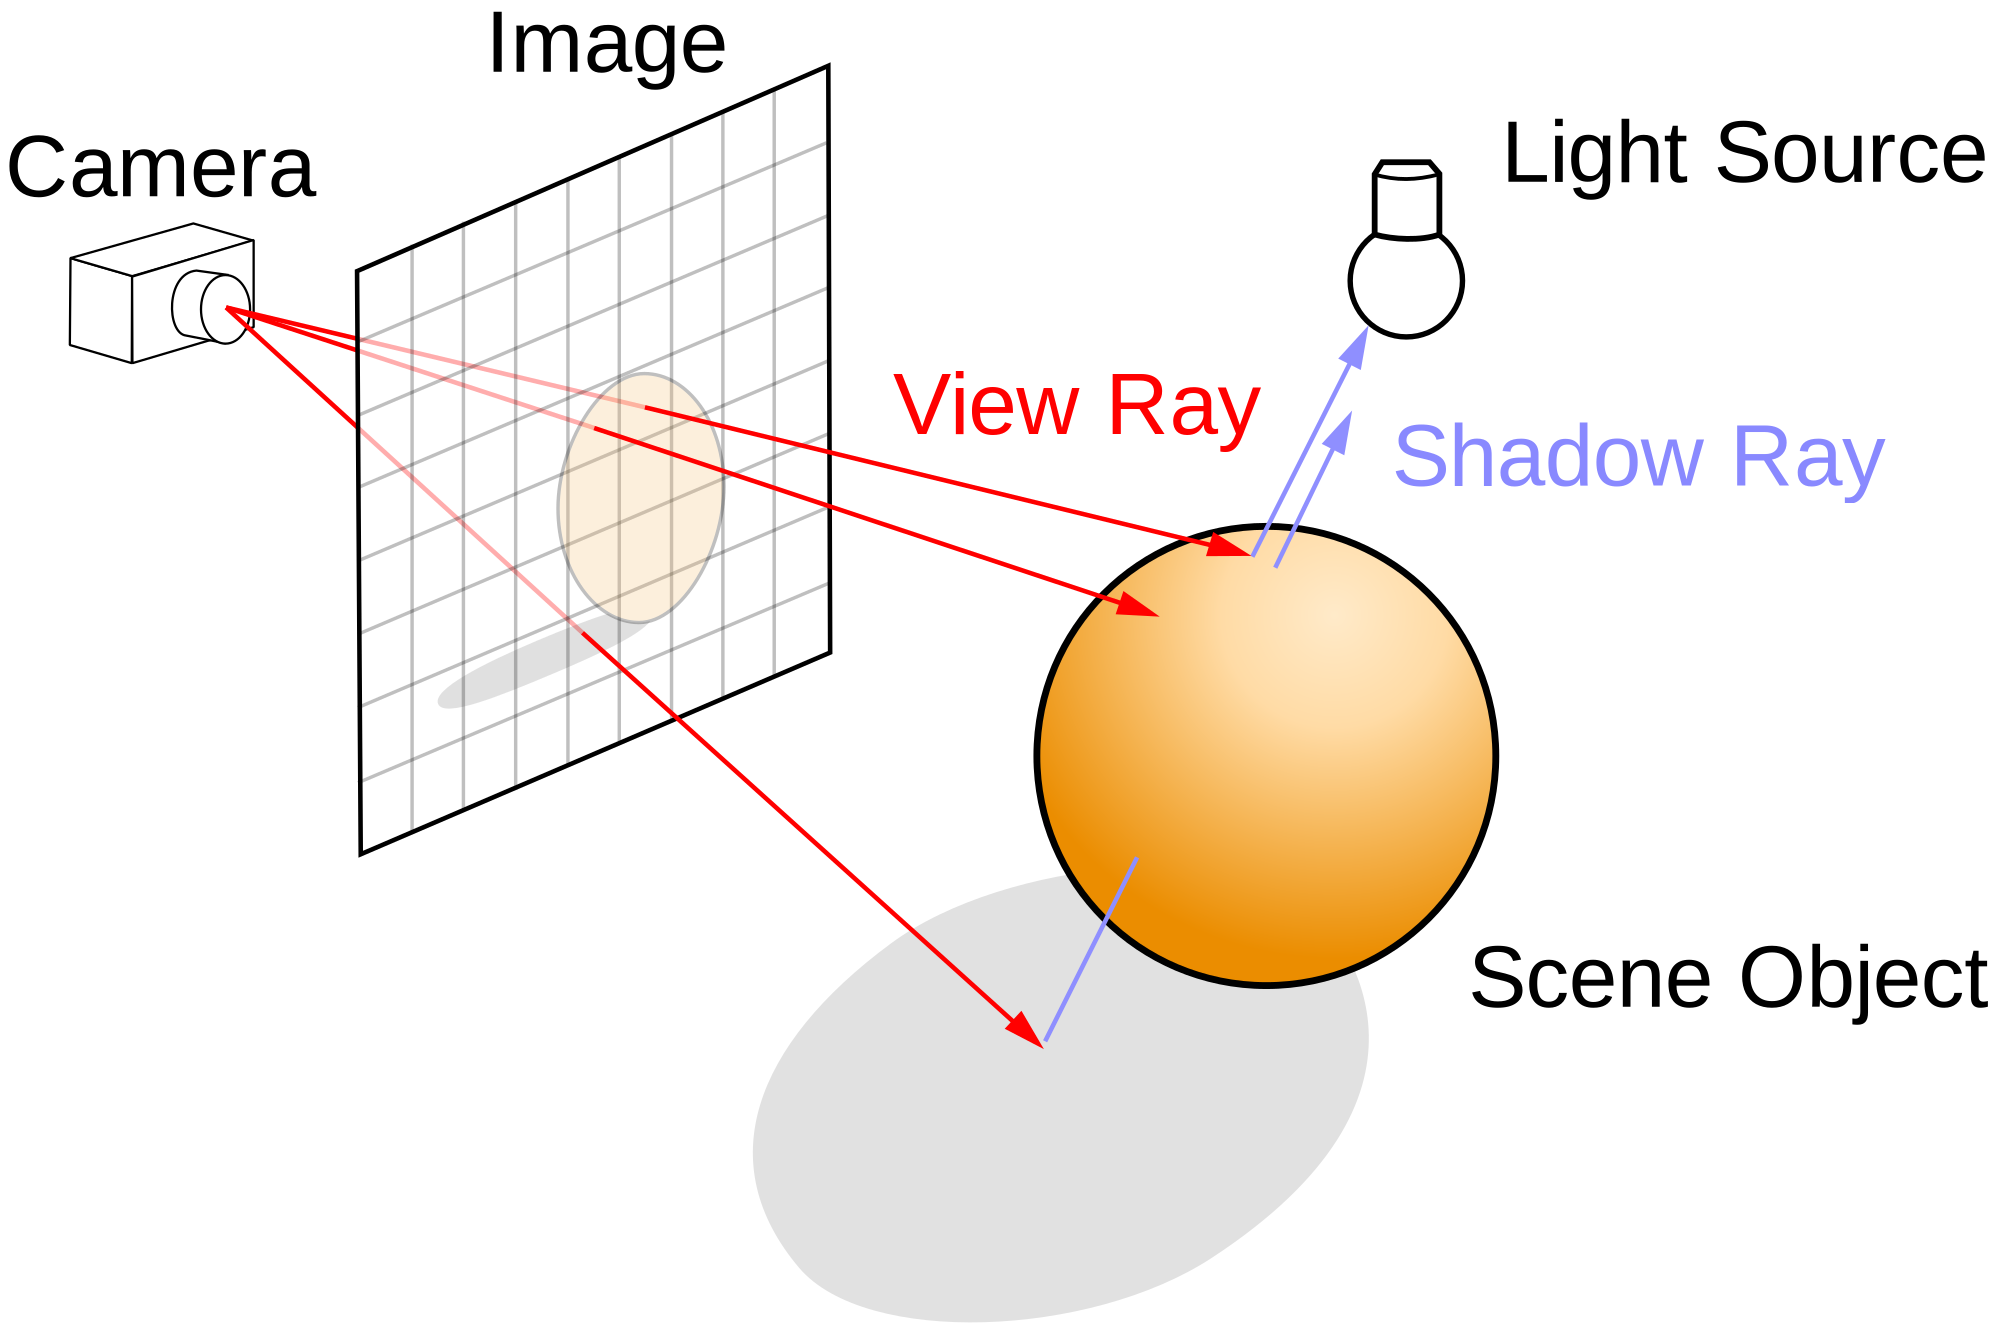
\includegraphics[width=0.6\textwidth]{images/Ray_trace_diagram.png}
        \caption{diagrama de raytracing}
        \label{fig:raytrace}
\end{figure}

A cena é representada como uma lista de formas, sendo que cada forma contém
uma lista de triângulos e o material que a constitui. Desta forma, para
encontrar os triângulos que um raio intersecta é necessário percorrer todas as
formas e todos os triângulos contidos na cena.

Uma implementação deste tipo apresenta um crescimento exponencial de tempo de
execução com o aumento da complexidade da cena fazendo com que seja fundamental
que algumas optimizações sejam aplicadas para melhorar a eficiência do
algoritmo.

\section{Paralelização Simples}

A primeira optimização realizada consiste em aplicar paralelismo simples ao
algoritmo inicial fazendo uso de \textit{std::thread}. Esta primeira
implementação de paralelismo baseia-se em lançar uma \textit{thread} para cada
linha da imagem com o objetivo que cada \textit{thread} calcule a sua respetiva
linha. Visto que cada pixel apenas é modificado por uma \textit{thread} e, por
isso, não existe concorrência ao nível do pixel, não é preciso qualquer tipo de
\textit{lock} para o \textit{array} que representa a imagem.

Este método já apresenta melhoria significativas de performance. No entanto, o
elevado número de \textit{threads} criadas em simultâneo (768 \textit{threads}
para ma imagem 1024x768) leva a \textit{high cpu contention} e a perdas de
performance.

\section{Paralelização com Queue}

Com o intuito de resolver o problema apresentado por serem lançadas demasiadas
\textit{threads} em simultâneo foi criada uma \textit{locked queue}.

Primeiro são lançadas N \textit{worker threads} (sendo N o numero de cores da
maquina em que esta a correr o código). Estas \textit{threads} lêem de uma
\textit{locked queue} qual é o trabalho que devem executar em seguida
finalizando a sua execução apenas quando a \textit{queue} estiver vazia. Cada
trabalho na \textit{queue} indica em que linha é que se deve começar a
renderizar e em que linha se deve acabar. Em seguida a \textit{queue} é
preenchida com todos os trabalhos necessários para
completar a imagem.

Esta optimização resolveu o problema de \textit{high cpu contention} criado pela
paralelização simples levando a um aumento significativo de performance.

\section{Flatten da Estrutura de Dados}

Com o objetivo de otimizar a estrutura de dados utilizada para representar uma
cena procedeu-se ao \textit{flatten} desta. Ou seja, em vez de se representar
sobre a forma de listas de formas, cada uma com uma lista de triângulos, passou
a se representar como uma lista de triângulos.

Apesar de esta implementação ser apenas um passo intermédio, também apresentou
um ligeiro aumento de performance.

\section{Bounding Volume Hierarchy}

Existem vários métodos para otimizar a procura de que triângulo um raio
interceta numa cena. Uma das mais utilizadas e a que foi explorada neste projeto
chama-se \textit{bounding volume hierarchy}. Este método consiste em converter a
estrutura de dados numa árvore, em que cada nodo contem um volume que engloba
todos os sub-nodos e que as folhas contém formas (Figura \ref{fig:bvh}).

\begin{figure}[h]
    \centering
        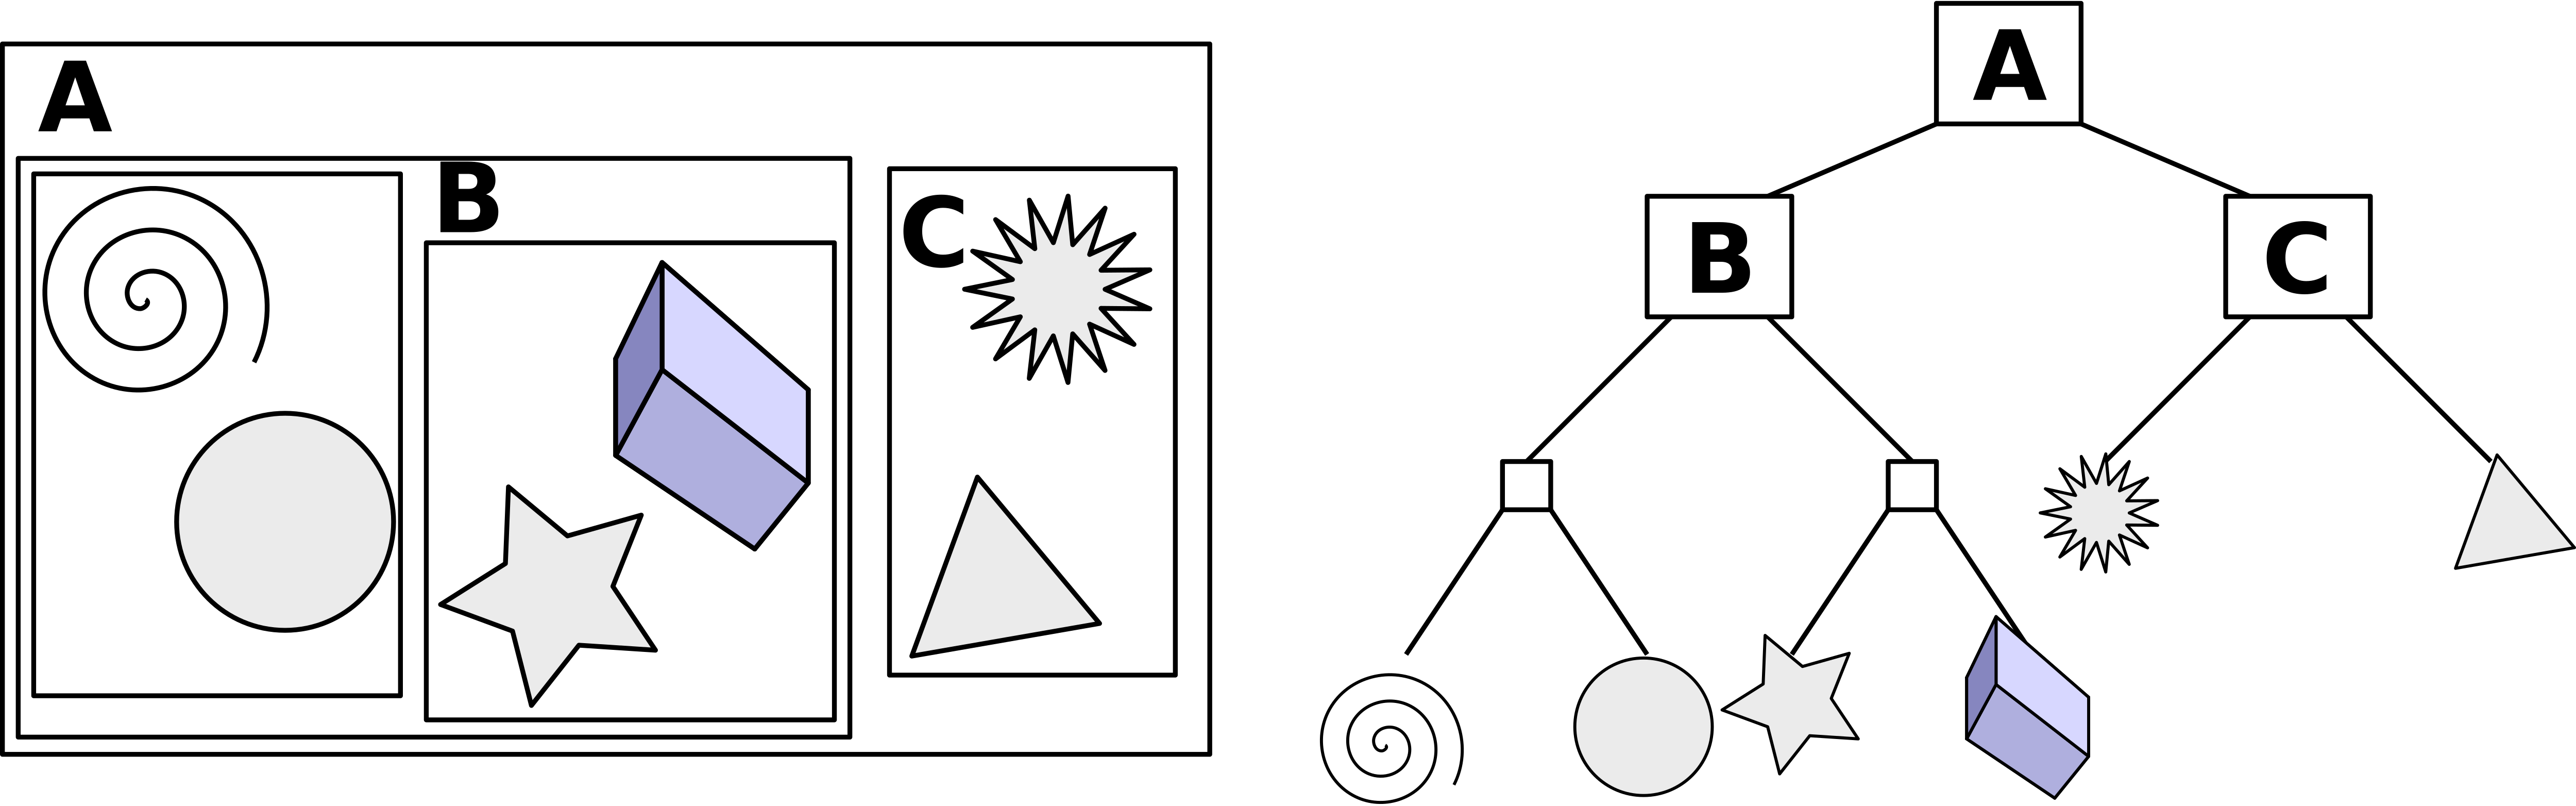
\includegraphics[width=0.8\textwidth]{images/bvh.png}
        \caption{Representacao de um BVH simples}
        \label{fig:bvh}
\end{figure}

O tipo de volume que foi escolhido denomina-se de \textit{axis aligned bounding
box}(AABB) em que as faces da caixa estão alinhadas com os eixos das coordenas.
Desta forma os cálculos feitos sobre estes volumes são mais simples e por isso
extremamente rápidos. E as formas que se encontram nas folhas da BVH são listas
de triângulos.

Para gerar esta árvore primeiro calcula-se a AABB que engloba todos os
triângulos da cena. Em seguida, divide-se essa caixa em 8 partes de volume
igual. Para cada uma desses volumes verifica-se quais são os triângulos que os
intersetam de alguma forma. Caso uma destas AABB não tenha nenhum triângulo
dentro é descartada, as que sobrarem são recursivamente divididas em 8 e o
processo repetido. Esta divisão termina quando o volume das caixas é demasiado
pequeno ou quando existe um numero baixo de triângulos dentro dela.

Assim, quando se pretende procurar qual é o triângulo dentro de uma cena que um
dado raio intersecta, apenas temos de para cada nodo verificar se o raio
intersecta os \textit{bounding volumes} dos sub-nodos, caso não intersecte esses
sub-nodos são completamente descartados. Desta forma não se tem de percorrer
todos os triângulos de uma cena de forma a encontrar o correto.

\section{Paralelização da Geração da BVH}

De forma a minimizar o impacto da criação da árvore no inicio do programa, foi
aplicada uma paralelização fazendo uso de \textit{std::async}.

Aquando da divisão de uma dada \textit{bounding box} é criada para cada uma
\textit{thread}. Esta divisão paralela apenas ocorre até um determinado nível da
árvore visto que se este limite não existisse iriam ser criadas demasiadas
\textit{threads} voltando a surgir o problema de \textit{high cpu contention}.

Depois de de ser feita a implementação deste novo algoritmo, constatou-se que
existiam artefactos que provavelmente advém de uma das AABB criadas com
\textit{std::async} ser perdida deixando uma falha na imagem. No código entregue
em anexo existe a função BVH::recursive\_parallel\_build no ficheiro
src/scene/scene.h que apresenta o que foi desenvolvido até ao momento.

\chapter{Comparação de Performance}

Todas as medidas de performance foram feitas utilizando o método \textit{k-best}
com k igual a 8 e utilizando o ficheiro \textit{CornellBox-Water.obj} (Figura
\ref{fig:water}).

\begin{figure}[h]
    \centering
        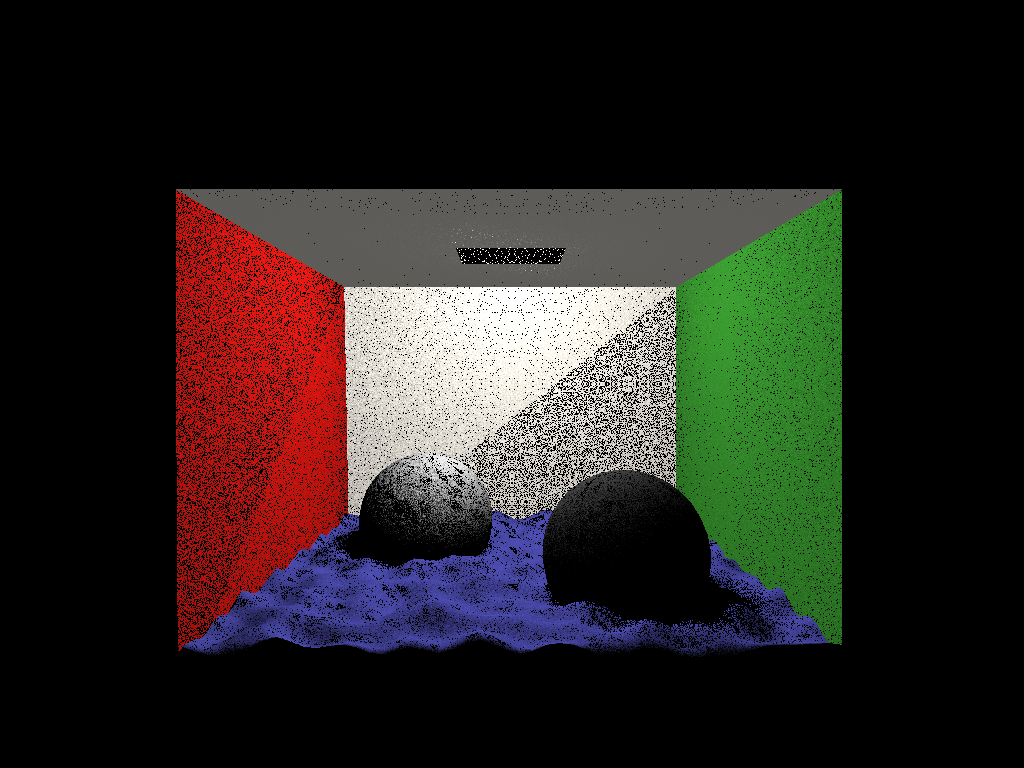
\includegraphics[width=0.8\textwidth]{images/water.png}
        \caption{Renderização de CornellBox-Water.obj}
        \label{fig:water}
\end{figure}

\begin{table}[h]
    \centering
    \begin{tabular}{|l|l|l|}
        \hline
                                      & tempo (ms) & speedup \\ \hline
        original                      & 99933      & 1.00x \\ \hline
        Paralelização Simples         & 46130      & 2.17x \\ \hline
        Paralelização com Queue       & 45207      & 2.21x \\ \hline
        Flatten da Estrutura de Dados & 43063      & 2.32x \\ \hline
        Bounding Volume Hierarchy     & 343        & 291.35x \\ \hline
    \end{tabular}
    \caption{Comparação de Performance da função de raytracer}
\end{table}

\begin{table}[h]
    \centering
    \begin{tabular}{|l|l|l|}
        \hline
                                  & tempo (ms) & speedup \\ \hline
        geração de BVH sequencial & 22     & 1.00x \\ \hline
        geração de BVH paralela   & -       & - \\ \hline
    \end{tabular}
    \caption{Comparação de Performance da geração de BVH}
\end{table}

Assim, fazendo uso de uma nova estrutura em forma de árvore para representar os
dados e paralelização com \textit{locked queue},  conseguiu-se obter um
\textit{speedup} de 291.35 vezes quando comparado com o algoritmo sequencial
original.

\end{document}
